\documentclass[a4paper,10pt]{scrartcl}
\usepackage[margin=2cm,bindingoffset=0cm]{geometry}
\usepackage{ucs}
\usepackage[utf8x]{inputenc}
\usepackage[ngerman]{babel}
\usepackage{fontenc}
%\usepackage[pdftex]{graphicx}
\usepackage{listings}
\usepackage{amssymb}
\usepackage{amsmath}
\usepackage{wasysym}
\usepackage{graphicx}
\usepackage[pdftex]{hyperref}
\author{Verena Käfer (2551188), Niklas Schnelle (2573250), Peter Vollmer (2553704)}
\date{erstellt am 25.10.2010\\
Version: 1.0}
\title{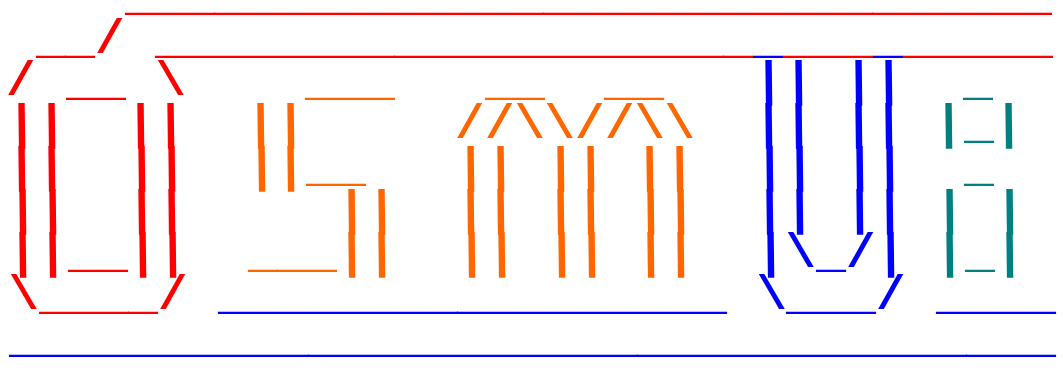
\includegraphics[width=15cm]{../projektplan/Logo_Osmui.png} \\ 
Spezifikation von OsmUi}

\begin{document}
\maketitle
\newpage
\tableofcontents
\newpage

\section{Einleitung}
\subsection{Zweck der Spezifikation}
Bei der Spezifikation handelt es sich um das zentrale Projektdokument. Sie ist Basis aller weiteren Dokumente und
Bezugspunkt in Funktionalitätsfragen. Sie ist daher unbedingt aktuell und konsistent zu halten.\\
Die Spezifikation beschreibt die Funktionen und Anforderungen an das Produkt OsmUi und das zugehörige Projekt.
\subsection{Leserkreis}
Diese Spezifikation richtet sich an:
\begin{itemize}
 \item Die Entwickler von OsmUi
 \item Den Kunden und die Betreuer des SoPra
\end{itemize}

\subsection{Projektüberblick}
In dem Entwicklungsprojekt OsmUi soll eine grafische Benutzeroberfläche für das Kommandozeilenwerkzeug \href{http://wiki.openstreetmap.org/wiki/Osmosis}{Osmosis}
entwickelt werden. Zu diesem Zweck überträgt OsmUi das abstrakte Pipelinekonzept von Osmosis auf eine grafische Darstellung, welche die gesamte
Funktionalität von Osmosis zugänglich macht, dabei aber deutlich benutzerfreundlicher sein soll.\\
Während bei Osmosis ein langer Kommandozeilenaufruf eine Pipeline zur Verarbeitung von OpenStreetMap Daten beschreibt, wobei sich der Benutzer die Befehle merken
und korrekt in der gewünschten Reihenfolge aufschreiben muss.\\
Soll es mit OsmUi möglich sein eine Verarbeitungspipeline ``zusammen zu klicken'' hierbei kann die Funktionsweise der einzelnen Tasks sowie deren Interaktion
der Benutzeroberfläche von OsmUi entnommen werden.
\subsection{Konventionen}

\section{Nichtfunktionale Anforderungen}
\subsection{Mengengerüst}
Bei OsmUi handelt es sich um eine Einzelplatzanwendung und es wird keine Netzwerkfunktion genutzt, somit gibt es zu jedem Zeitpunkt einen Nutzer.\\
Beim erstellen/laden/speichern von Verarbeitungspipelines muss OsmUi in der Lage sein mit Pipelines von bis zu 100 Tasks zuverlässig zu arbeiten,
eine künstliche Beschränkung nach oben besteht jedoch nicht.
\subsection{Entwurfseinschränkungen}
\subsubsection{Entwurfskonzept}
OsmUi wird nach dem \href{http://de.wikipedia.org/wiki/KISS-Prinzip}{KISS-Prinzip} entwickelt, d.h. entscheidend für die Qualität der Software soll
sein wie gut die Hauptfunktionen unterstützt werden, bessere Hauptfunktionalität ist einem größeren Funktionsumfang unterzuordnen.\\
Im Fall von OsmUi heißt dies, dass das Hauptaugenmerk auf dem einfachen und sinnvollen erstellen von Verarbeitungspipelines, deren Import und Export liegt.
Weniger wichtig sind hingegen ``Luxusfunktionen'' wie direktes Anzeigen des Verarbeitungsergebnisses (was auf Grund der Vielfalt der Funktionen von Osmosis
und der Verarbeitungsdauer onehin nicht immer sinnvoll ist) oder das direkte Aufrufen von Osmosis.
\subsubsection{Systemumgebung}
Systemumgebung ist das \textbf{Java Runtime Environment in Version 1.6 und höher (SE)}. Dabei ist OsmUi als reine Java Anwendung zu entwickeln, so dass
keine externen Abhängigkeiten bestehen und OsmUi auf allen Java SE Kompatiblen Systemen eingesetzt werden kann.
Eventuell wird intern die Bibliothek \textbf{JGraph} eingesetzt, diese wird dann aber direkt mit ausgeliefert
und ist ebenfalls reines Java. 
\subsubsection{Layout und Gestaltung}
OsmUi soll ab einer Auflösung von 1024x768 benutzbar sein. Alle Fenster sollen, wenn dies sinnvoll ist skalierbar sein und den eventuell gewonnen Platz sinnvoll
nutzen. Um Benutzer von Multimonitorsystemen und exotischen Windowmanagern zu entlassen soll die Positionierung von neuen Fenstern nativ erfolgen, d.h. es
sollen insbesondere keine Fenster in eine errechnete Bildschirmmitte von OsmUi selbst positioniert werden.
\subsection{Robustheit}
OsmUi soll als Software möglichst robust arbeiten, d.h. unter allen Bedinungen korrekt arbeiten. Dies soll durch defensive Programmierung erreicht werden.
Jedoch sollen Benutzereingaben möglichst früh geprüft werden, so dass tiefere Funktionen den Daten ``vertrauen'' können, dies sichert zudem ab, dass klar ist, welcher
Programmteil für die Prüfung zuständig ist, nämlich immer der erste der die nötigen Informationen hat.\\
Weiterhin wird die Robustheit durch das KISS-Prinzip unterstützt indem weniger Funktionen besser entworfen und getestet werden können.
\subsection{Portabilität}
OsmUi soll durch den Einsatz reinen Java's auf alle Systeme mit Java SE 1.6 Unterstützung lauffähig sein. Als Exportformate für Osmosis Kommandoscripts
werden .bat und .sh (/bin/sh) Unterstützt womit alle Posix Systeme sowie Windows abgedeckt sind.
\subsection{Erweiterbarkeit}
Das Programm muss keine besonderen Erweiterungsfunktionalitäten wie etwa ein Pluginsystem zur Verfügung stellen, jedoch wird der Programmcode und die Systemarchitektur
so gestaltet, dass OsmUi leicht und schnell an neue oder veränderte Osmosis Funktionen angepasst werden kann.
\subsection{Distributionsform und Installation}
OsmUi wird als ausführbares JAR Archiv ausgeliefert, welches auf allen Java SE 1.6 fähigen Systemen benutzt werden kann. Gegebenenfalls wird es außerdem Pakete 
für einige Linux Distributionen geben, die die Installation erleichtern sowie OsmUi in Menüs einbinden.
\section{Akteure}
\subsection{Benutzer}
Bei OsmUi gibt es grundsätzlich nur eine Nutzerklasse. Es wird davon ausgegangen, dass OsmUi benutzt wird um eine Verarbeitungspipeline für OpenStreetMap Daten
zu erstellen, welche anschließend durch Osmosis ``ausgeführt'' wird. Hierbei wird davon ausgegangen, dass der Nutzer grundlegende Kentnisse 
von Datenverarbeitung und OpenStreetMap hat.
\section{Laden und Speichern von Verarbeitungspiplines als Osmosis Aufrufscript}
Dem KISS-Prinzip folgend bietet OsmUi eine einheitliche Laden und Speichern Funktion, die sowohl eventuell bereits vorhandene Osmosis Aufrufscripts
laden kann, als auch durch OsmUi selbst erstellte Verarbeitungspiplines, die immer auch als Aufrufscript gespeichert werden. 
Dies ermöglicht auch beim Wechsel des Werkzeugs einen leichten Zugriff auf alle mit OsmUi erstellten Dateien.
\subsection{Laden}
Eine der Hauptfunktionen von OsmUi stellt das Laden von Aufrufscripten da. Dabei können sowohl Dateien im .bat, als auch im .sh Format (mit \#!/bin/sh Shebang)
sowie Textdateien in denen nur eine Osmosis Parameterliste steht geladen werden. Sie werden direkt im Pipelinebearbeitungsfeld angezeigt und
stehen zur Bearbeitung bereit.
\subsubsection{Speichern}
Zum Speichern wählt der Benutzer entweder einen neue Datei aus, die wenn vorhanden überschrieben und sonst neu erstellt wird, oder er überschreibt die gerade bearbeitete Datei.
Der Dateityp kann hierbei zwischen .sh Script und .bat gewählt werden, wobei die zu letzt verwendete Einstellung der voreingestellt ist.
\section{Benutzeroberfläche}
Die Benutzeroberfläche von OsmUi ist in zwei Hauptteile aufgeteilt, zudem gibt es ein Anwendungsmenü. Im linken Teil können neue Tasks ausgewählt werden die zur
Pipeline hinzugefügt werden können.
\section{Lokalisation}
OsmUi wird Lokalisation für mindestens Deutsch und Englisch bieten. Dabei wird die aktuelle Sprache aus den hierfür vorgesehenen Umgebungsvariablen eingelesen um
sie ohne Interaktion durch den Benutzer in dessen System ein zu gliedern.
%\subsection{Titelleiste des Hauptfensters}
%\subsection{Startbildschirm}
%\subsection{Moduswahlbildschirm}
%\subsection{Allgemeine Beschreibung des Hauptfensters}
%\subsubsection{Die Modusleiste}
% \subsubsection{Verhalten bei Änderung der Fenstergröße}
% \subsubsection{Verhalten von Rückgängig und wiederholen}\subsection{Titelleiste des Hauptfensters}
% \subsection{Startbildschirm}
% \subsection{Moduswahlbildschirm}
% \subsection{Allgemeine Beschreibung des Hauptfensters}
% \subsubsection{Die Modusleiste}
% \subsubsection{Verhalten bei Änderung der Fenstergröße}
% \subsubsection{Verhalten von Rückgängig und wiederholen}
% \subsubsection{Verhalten beim Erstellen von Kopien}
% \subsubsection{Verhalten beim Entfernen von Elementen}
% \subsubsection{Filterung der Auswahl beim Duplizieren, Kopieren und Verschieben}
% \subsection{Menübefehle}
% \subsubsection{Alle Testsequenzen exportieren}
% \subsubsection{Ausschneiden}
% \subsubsection{Ausgewählte Testsequenz exportieren}
% \subsubsection{Auswertung}
% \subsubsection{Beenden}
% \subsubsection{Benutzerverwaltung}
% \subsubsection{Durchführung}
% \subsubsection{Einfügen}
% \subsubsection{Einstellungen}
% \subsubsection{\textit{Elememt} an das Ende verschieben}
% \subsubsection{\textit{Element} an den Anfang verschieben}
% \subsubsection{\textit{Element} eine Position nach ob}
% \subsubsection{\textit{Element} eine Position nach unten}
% \subsubsection{\textit{Element} duplizieren}
% \subsubsection{\textit{Element} entfernen}
% \subsubsection{Hilfe}
% \subsubsection{Kopieren}
% \subsubsection{Neue Testsequenz}
% \subsubsection{Neuer Testfall}
% \subsubsection{Neues Projekt}
% \subsubsection{Programmfehler melden}
% \subsubsection{Projekt öffnen}
% \subsubsection{Projekt schließen}
% \subsubsection{Projekt speichern}
% \subsubsection{Projekt speichern unter}
% \subsubsection{Rückgängig}
% \subsubsection{Suchen}
% \subsubsection{Test abbrechen}
% \subsubsection{Test durchführen}
% \subsubsection{Testdaten importieren}
% \subsubsection{Testprotokoll als PDF speichern}
% \subsubsection{Über}
% \subsubsection{Update Prüfung}
% \subsubsection{Verwaltung}
% \subsubsection{Wiederholen}
% \subsubsection{Zuletzt geöffnete Projekte}
% \subsection{Gliederung der Menüleiste}
% \subsection{Hauptfenster im Verwaltungsmodus}
% \subsubsection{Der Baum}
% \subsubsection{Inhaltsbereich mit Mehrfachausahl oder ohne Auswahl im Baum}
% \subsubsection{Inhaltsbereich bei Auswahl einer Testsequenz}
% \subsubsection{Inhaltsbereich bei Auswahl eines Testfalls}
% \subsubsection{Verhalten der Eingabefelder im Inhaltsbereich}
% \subsection{Hauptfenster im Durchführungsmodus}
% 
% \subsubsection{Verhalten beim Erstellen von Kopien}
% \subsubsection{Verhalten beim Entfernen von Elementen}
% \subsubsection{Filterung der Auswahl beim Duplizieren, Kopieren und Verschieben}
% \subsection{Menübefehle}
% \subsubsection{Alle Testsequenzen exportieren}
% \subsubsection{Ausschneiden}
% \subsubsection{Ausgewählte Testsequenz exportieren}
% \subsubsection{Auswertung}
% \subsubsection{Beenden}
% \subsubsection{Benutzerverwaltung}
% \subsubsection{Durchführung}
% \subsubsection{Einfügen}
% \subsubsection{Einstellungen}
% \subsubsection{\textit{Elememt} an das Ende verschieben}
% \subsubsection{\textit{Element} an den Anfang verschieben}
% \subsubsection{\textit{Element} eine Position nach ob}
% \subsubsection{\textit{Element} eine Position nach unten}
% \subsubsection{\textit{Element} duplizieren}
% \subsubsection{\textit{Element} entfernen}
% \subsubsection{Hilfe}
% \subsubsection{Kopieren}
% \subsubsection{Neue Testsequenz}
% \subsubsection{Neuer Testfall}
% \subsubsection{Neues Projekt}
% \subsubsection{Programmfehler melden}
% \subsubsection{Projekt öffnen}
% \subsubsection{Projekt schließen}
% \subsubsection{Projekt speichern}
% \subsubsection{Projekt speichern unter}
% \subsubsection{Rückgängig}
% \subsubsection{Suchen}
% \subsubsection{Test abbrechen}
% \subsubsection{Test durchführen}
% \subsubsection{Testdaten importieren}
% \subsubsection{Testprotokoll als PDF speichern}
% \subsubsection{Über}
% \subsubsection{Update Prüfung}
% \subsubsection{Verwaltung}
% \subsubsection{Wiederholen}
% \subsubsection{Zuletzt geöffnete Projekte}
% \subsection{Gliederung der Menüleiste}
% \subsection{Hauptfenster im Verwaltungsmodus}
% \subsubsection{Der Baum}
% \subsubsection{Inhaltsbereich mit Mehrfachausahl oder ohne Auswahl im Baum}
% \subsubsection{Inhaltsbereich bei Auswahl einer Testsequenz}
% \subsubsection{Inhaltsbereich bei Auswahl eines Testfalls}
% \subsubsection{Verhalten der Eingabefelder im Inhaltsbereich}
% \subsection{Hauptfenster im Durchführungsmodus}
\end{document}
